%% elec6530_final.tex
%% 2011/11/14
%% by William J. Woodall IV
%% and John Harrison

\documentclass[journal]{IEEEtran}

%% For Citations
\usepackage{cite}

%% For graphics
\usepackage[pdftex]{graphicx}
\graphicspath{{images/}}
\DeclareGraphicsExtensions{.pdf,.jpeg,.png}

%% For URL's
\usepackage{url}

% correct bad hyphenation here
\hyphenation{op-tical net-works semi-conduc-tor}

\begin{document}
  
  \title{Simulated Path Planning for Auburn's Autonomous Lawnmower}
  
  \author{John~Harrison~and
          William~J.~Woodall~IV% <-this % stops a space
  
  % Thanks
  % \thanks{Dr. Thaddeus A. Roppel}}
  }
  
  % Paper Header
  \markboth{ELEC 5530/6530 Introduction to Autonomous Mobile Robotics}%
  {Woodall and Harrison:Simulated Path Planning for Auburn's Autonomous Lawnmower}
  
  % Make room for the title
  \maketitle
  
  % Abstract
  \begin{abstract}
    Auburn University has a competition Autonomous Lawnmower team and competes
    every year at ION's competition\cite{IONAutomow} in Dayton, OH.  This
    paper describes the how the team has approached coverage path planning for 
    the lawnmower given the competition constraints.  The competition setting 
    dictates a closed polygon filed, which can be concave, and it will contain 
    several static and dynamic obstacles.  The path planner for the lawnmower 
    has to navigate this field while covering as much as the field as possible 
    and without competition field specific knowledge.  The algorithm 
    implemented here have results that resemble the output of the 
    Boustrophedon Cellular Decomposition\cite{Choset_1997_1416} method.  The 
    paper describes the implementation of this algorithm and some 
    examples of its performance in different situations.  Additionally, the 
    paper shows the simulation environment setup in the two dimensional, 
    kinematic robotics simulator, Stage\cite{vaughan2000stage}.
  \end{abstract}
  
  % Keywords
  \begin{IEEEkeywords}
    Coverage Path Planning, Mobile Robotics, Navigation, Simulation
  \end{IEEEkeywords}
  
  % Don't know if I need this...
  \IEEEpeerreviewmaketitle
  
  \section{Introduction}
  \IEEEPARstart{C}{overage} path planning determines a path that guarantees coverage of an area in an admissible manner for the agent.  This type of path planning can be applied to many areas of work including detection of unexploded ordinance, floor cleaning, or crop plowing, just to name a few. In the case of this paper the application is lawn-mowing, the agent is Auburn's Autonomous Lawnmower, and the area is the competition field.  Though this paper sticks to these constraints the implementation here should be generalized enough to be easily applied to other applications or situations.  This paper assumes a few other things about the environment.  First, the assumption is made that this planning is done off-line with knowledge about the area to be covered and the obstacles in the environment.  This means that there is no planned dynamic obstacle avoidance at this point.  The previous competition year's field, which was surveyed with RTK GPS equipment, will be used as a test shape during this paper.
  
  Optimally, the path should contain as few turns as possible, but irregular shapes, shapes with odd angles and interior obstacles, pose problems for generating an optimal path. Minimizing the turns, would improve cutting quality and to avoid short comings of the navigation system. To find the path with the fewest number of turns for a regular shape such as a rectangle, the simplest way is to find the longest edge and generate paths that are parallel to that edge. For other shapes, such as an ellipses, following parallel the longest edge of the bounding box will produce the best path with the fewest turns. More complex shapes require cellular decomposition to find an optimal path for a given cell. Breaking each component of the shape into semi-regular cells can help break down the problem into smaller portions for generating the optimal path.\cite{1307193}
  
  \section{Description of the Algorithm}
  In this section of the paper we will describe the algorithm that will be used on the Autonomous Lawnmower for path planning.  The basic coverage ``shape'' is called the Boustrophedon path, which literally means ``the way of the ox.''\cite{Choset_1997_1416}  As previously stated the resulting coverage path resembles the output of a Boustrophedon Cellular Decomposition in that it covers each cell of the area in order, but at no point during this implementation of the algorithm is the cellular decomposition formally done.  This effect is just a product of the manner in which the algorithm selects the order of waypoints to be traveled to.
  
  \begin{figure}[here]
    \centering
    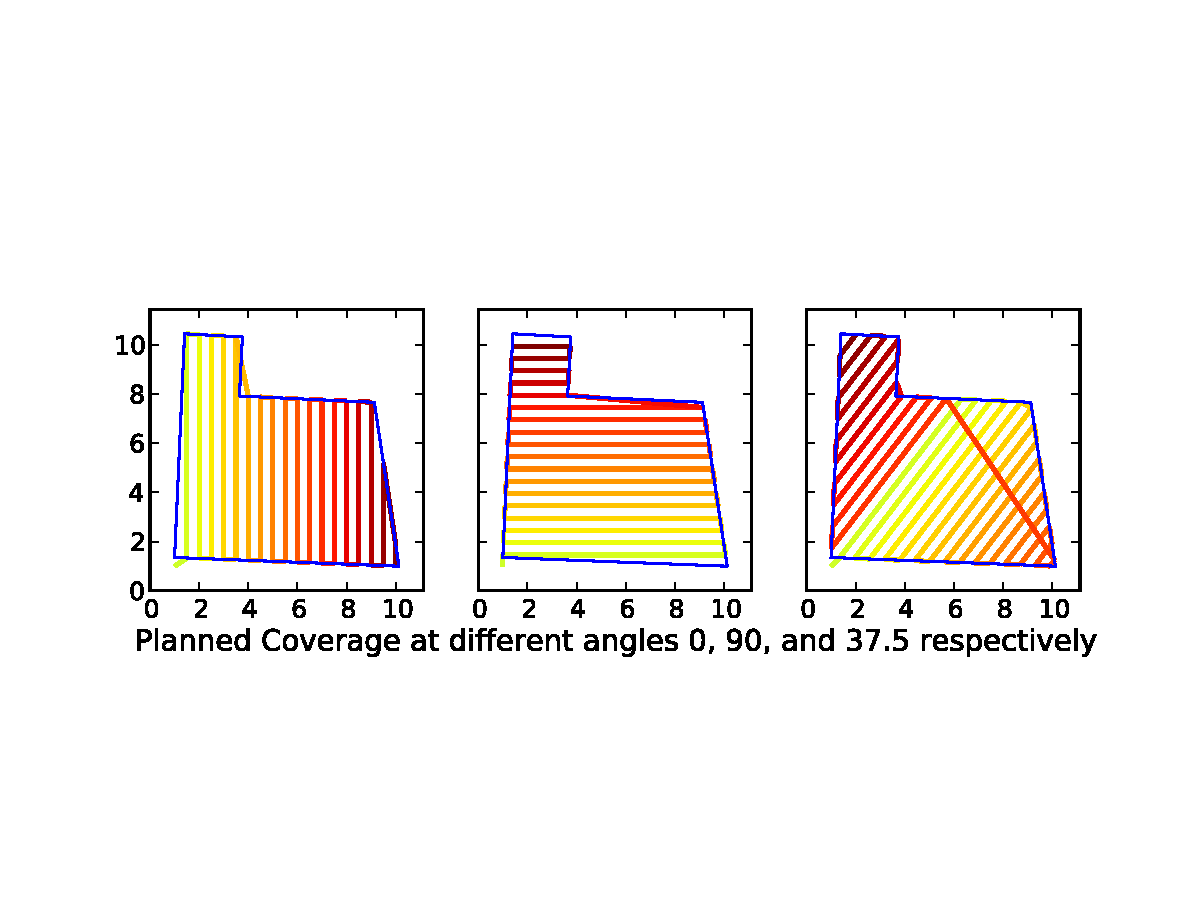
\includegraphics[width=3.75in,keepaspectratio]{rotations.pdf}
    \caption{Different Cutting Rotations}
    \label{fig:rotations}
  \end{figure}
  
  \subsection{Field Rotation}
  One of the parameters of our algorithm is the angle at which the ``cutting lines'' are set.  You can see in Figure~\ref{fig:rotations} that this algorithm can plan and coverage at angle specified angle.  This allows us to pick, offline, the best cutting direction for a given field.  There are also some tools for automatically picking the best angle of cutting and starting point.  Figure~\ref{fig:longest_edge} shows how the angle of the longest edge has been selected automatically as the cutting angle.  Other heuristics or methods could be used to determine the best angle of cutting.  In order to simplify the work in generating a path that adheres to the cutting angle, the field polygon's points are simply rotated into a frame where the cutting angle is along the y axis.  The map is rotated into the cutting angle frame using rotation matrices\cite[p.60]{siegwart2004introduction}, such that each point map polygon is multiplied by the inverse rotation matrix given by:
  
  $$R\left( \theta  \right)^{-1}\; =\; \left[ \begin{array}{ccc} \cos \left( \theta  \right) & -\sin \left( \theta  \right) & 0 \\ \sin \left( \theta  \right) & \cos \left( \theta  \right) & 0 \\ 0 & 0 & 1 \end{array} \right]$$
  
  Where $\theta$ is the angle of cutting specified.  After applying the rotation to the field then the planning can assume vertical lines intersecting the field will produce the desired cutting lines.  Once the planning is complete, the resulting waypoints of the path are each multiplied by the forward rotation matrix given by:
  
  $$R\left( \theta  \right)\; =\; \left[ \begin{array}{ccc} \cos \left( \theta  \right) & \sin \left( \theta  \right) & 0 \\ -\sin \left( \theta  \right) & \cos \left( \theta  \right) & 0 \\ 0 & 0 & 1 \end{array} \right]$$
  
  Again, with $\theta$ representing the angle of cut.  This puts the path back into the map frame.
  
  \begin{figure}[here]
    \centering
    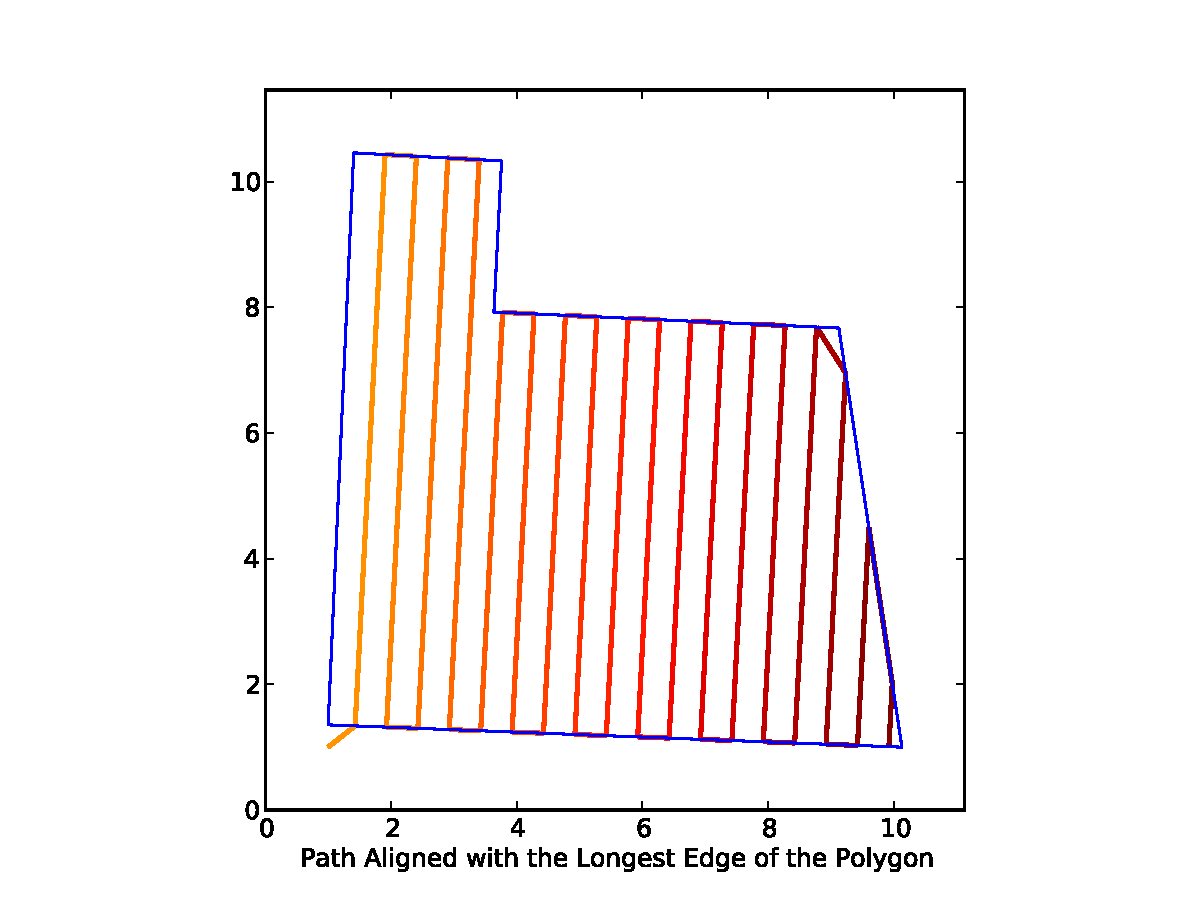
\includegraphics[width=3.5in,keepaspectratio]{longest_edge.pdf}
    \caption{Cutting Angle Parallel with the Longest Edge}
    \label{fig:longest_edge}
  \end{figure}
  
  \subsection{Finding Intersection Points}
  Once the map polygon has been transformed into the cutting angle frame then the map is ready to be intersected by vertical lines.  The first vertical line is the vertical line that is collinear with the point or points of the map that have the smallest x value.  This gives the left most vertical line that intersects the map polygon.  The right most line, which is the left most line on the first iteration, is expanded to the right by $1/2$ of the cutting width and then the intersecting points between the new expanded line and map polygon are put into a list of points to visit.  This is continued until the new expanded line does not intersect the map polygon.  This can be visualized in Figure~\ref{fig:intersections}, where the solid red line is the first intersection line and the solid black lines are the intersection lines to follow.
  
  \begin{figure}[here]
    \centering
    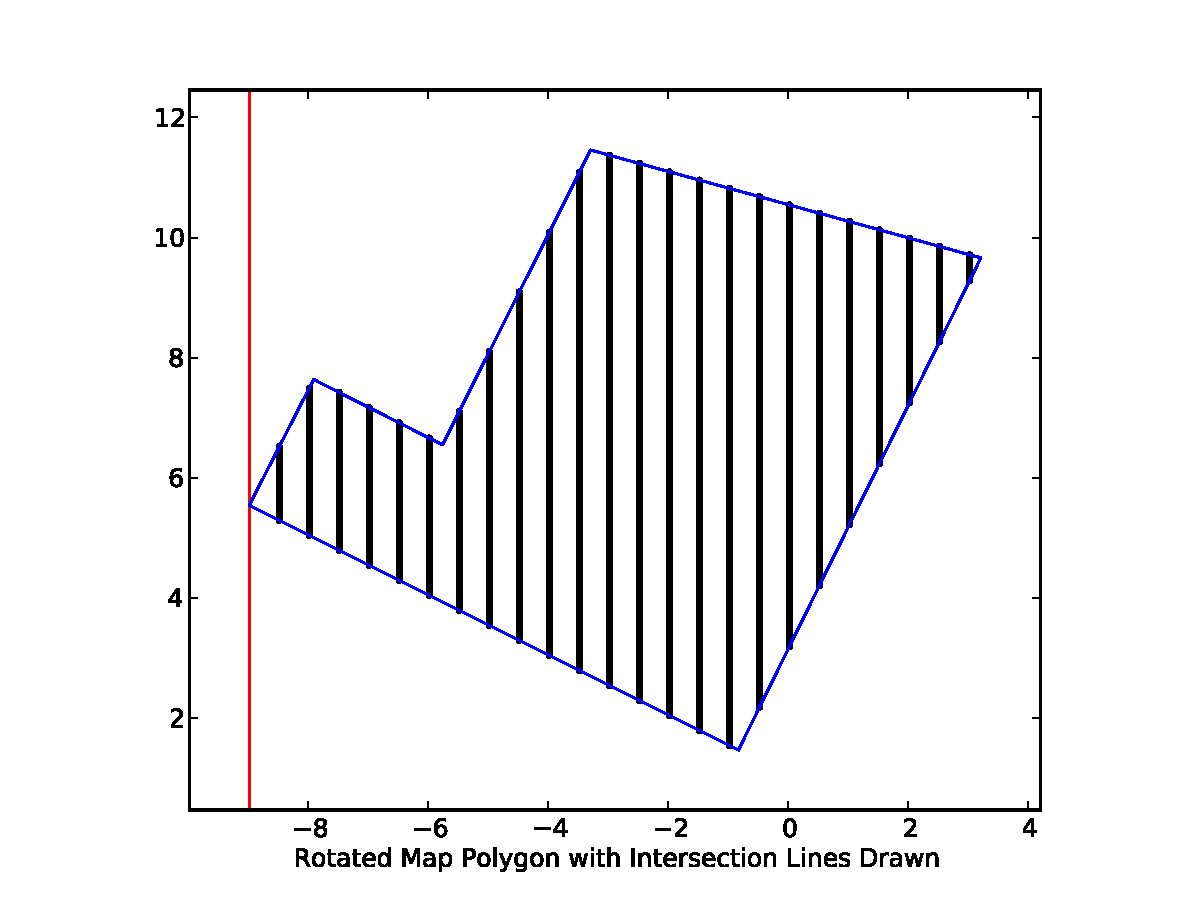
\includegraphics[width=3.5in,keepaspectratio]{intersection.pdf}
    \caption{Intersection Lines Drawn on a Rotated Map Polygon}
    \label{fig:intersections}
  \end{figure}
  
  \subsection{Ordering Intersection Points}
  Once the intersection points have been found from the intersection lines and the map polygon, those points need to be ordered.  The algorithm for ordering those path points starts by finding the closest point to the origin, also referred to as the starting position, and that point is set to the current point.  Then the algorithm follows the intersection line associated with the current point till it reaches the matching point on the opposite side and that becomes the current point.  Then the closest point of the closest intersection line in the positive x direction is set to the current point.  This is repeated until all points have been visited.  Each time a new current point is set, the previous current point is appended to an ordered list.  This list becomes the path once all of the points have been visited.  Finally, the points in the path are each rotated back into the map frame and are ready to be fed to the controller as waypoints.
  
  \begin{figure}[here]
    \centering
    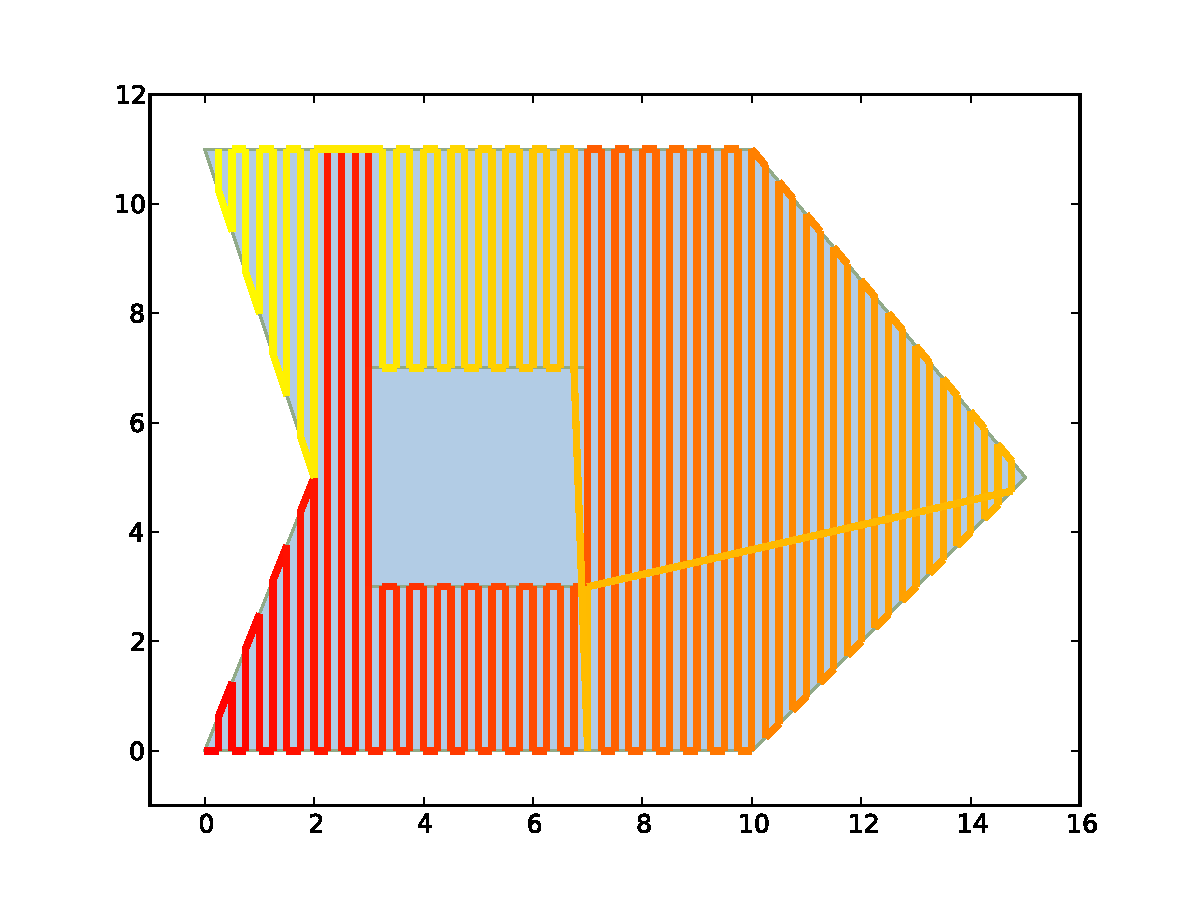
\includegraphics[width=3.5in,keepaspectratio]{obstacle.pdf}
    \caption{Coverage Planning with Concave Map Polygon and a Static Obstacle}
    \label{fig:obstacle}
  \end{figure}
  
  \begin{figure}[here]
    \centering
    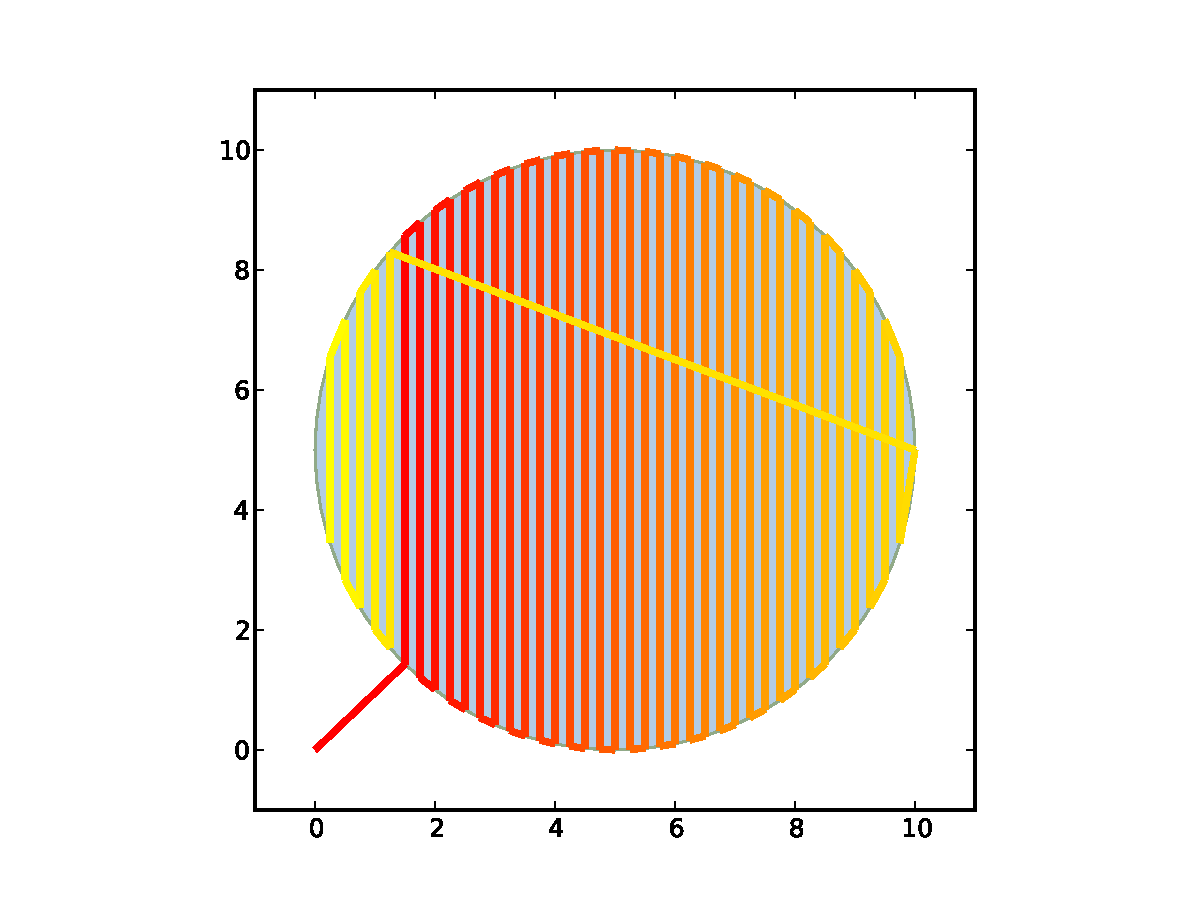
\includegraphics[width=3.5in,keepaspectratio]{circle.pdf}
    \caption{Coverage Planning on a Circular Map Polygon}
    \label{fig:circle}
  \end{figure}
  
  \section{Results}
  It has already been shown that the coverage planner can allow for different cutting angles and starting points, and that it can successfully plan even with concave shapes.  In this section of the paper we will show that it can handle many edge cases.  Figure \ref{fig:obstacle} shows that the path planner can handle concave shapes that have the concave alcove against the grain of the path planner.  It also shows that the planner can deal with known static obstacles.  Figure \ref{fig:circle} shows that the coverage planner can handle irregular map polygon shapes like circular shapes.
  
  \section{Simulation with Stage}
  To simulate the use of the path planner and the controller together the competition environment was setup in the two dimensional simulator called Stage\cite{vaughan2000stage}.  Stage allows the simulated robot to interact with the path planner, obstacles detection and avoidance system, and the controller as if it were the real system.  The communication and runtime is all handled through the Robotic Operating System, ROS\cite{quigley2009ros}.  There is very little interaction with the path planner described in this paper and the simulator, but the work following this that allows for on-line obstacle detection and avoidance will need to interface with the simulator.  The controller could be show in the simulator, but it is still currently in Matlab being tuned so that is not possible at this time.
  
  \begin{figure}[here]
    \centering
    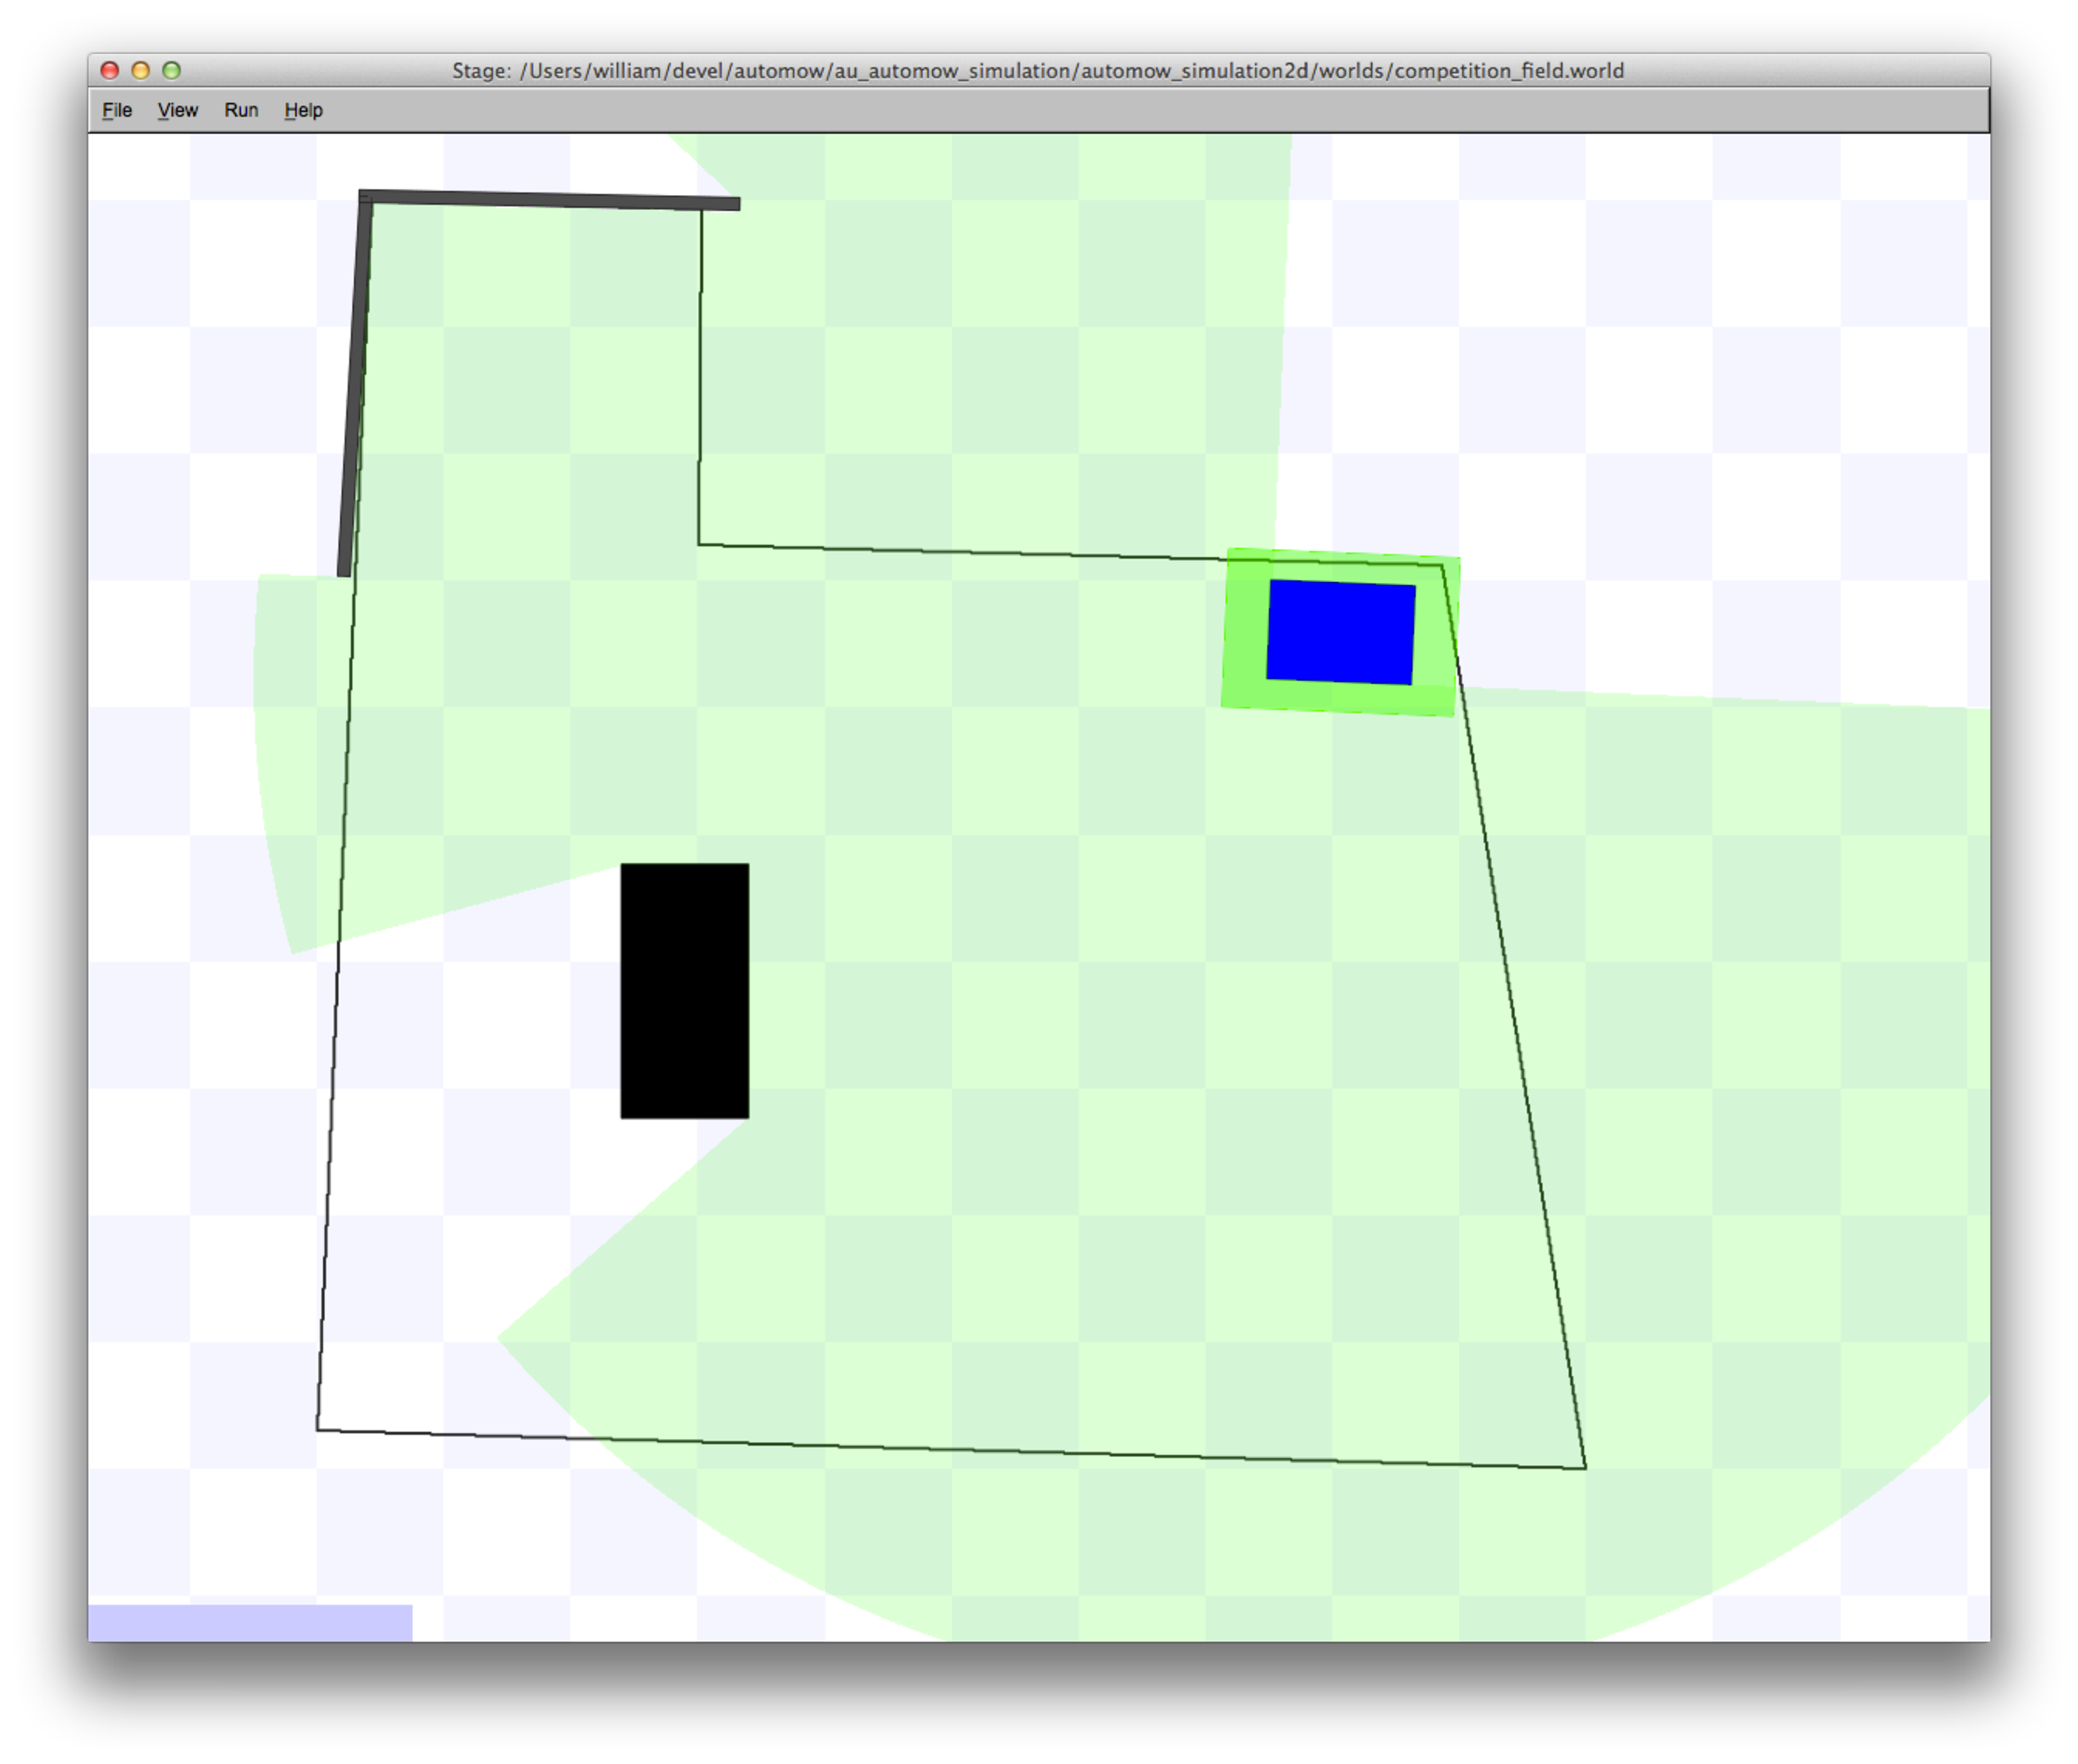
\includegraphics[width=3.5in,keepaspectratio]{stage.pdf}
    \caption{Stage World that Models the Competition and Lawnmower}
    \label{fig:stage}
  \end{figure}
  
  \section{Future Work}
  The output of the planner needs to be mapped into the controller to ensure that the controller is capable of performing the requested path.  Currently the planner requires off-line knowledge of the field shape and obstacles.  In the future the planner should incorporate the ability to detect and avoid obstacles in real-time to handle obstacles that cannot be measured off-line or dynamic obstacles.  Finally, it would be interesting to try and run the coverage planning from a situation where nothing is known about the survey area.  Input from sensors like vision and laser range finders would be required to find the boundaries of the map.
  
  \section{Conclusion}
  This paper has introduced a coverage path planning system tailored to the Autonomous Lawnmower Competition, but that has a general solution that can be applied to many situations and platforms.  The coverage planner in this paper should provide a sufficient system for planning an admissible path for the Autonomous Lawnmower project to proceed with testing and integration.
  
  \newpage
  
  \bibliographystyle{IEEEtran}
  \bibliography{citations}
  
  \begin{IEEEbiography}[{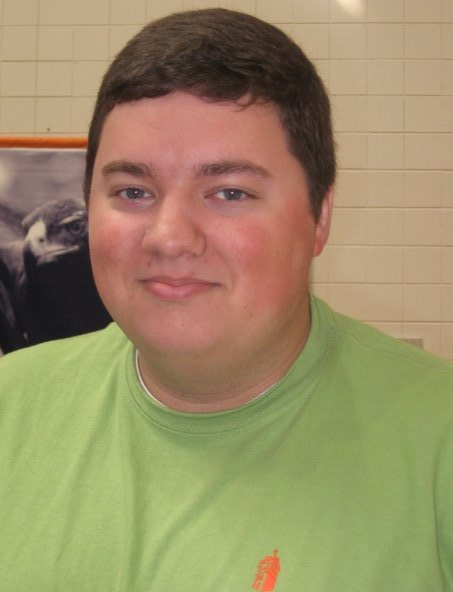
\includegraphics[width=1in,height=1.25in,clip,keepaspectratio]{william.jpg}}]{William J. Woodall IV}
  William is a graduate research assistant at Auburn University and is 
  pursuing his Master of Science in Software Engineering.  He works for Dr. 
  David Bevly of the Mechanical Engineering Department on Mobile Robotics and 
  Advanced Teleoperation.  William's research interests include mobile 
  robotics, navigation and control, and perception.  \url{http://williamjwoodall.com}
  \end{IEEEbiography}
  
  \begin{IEEEbiography}[{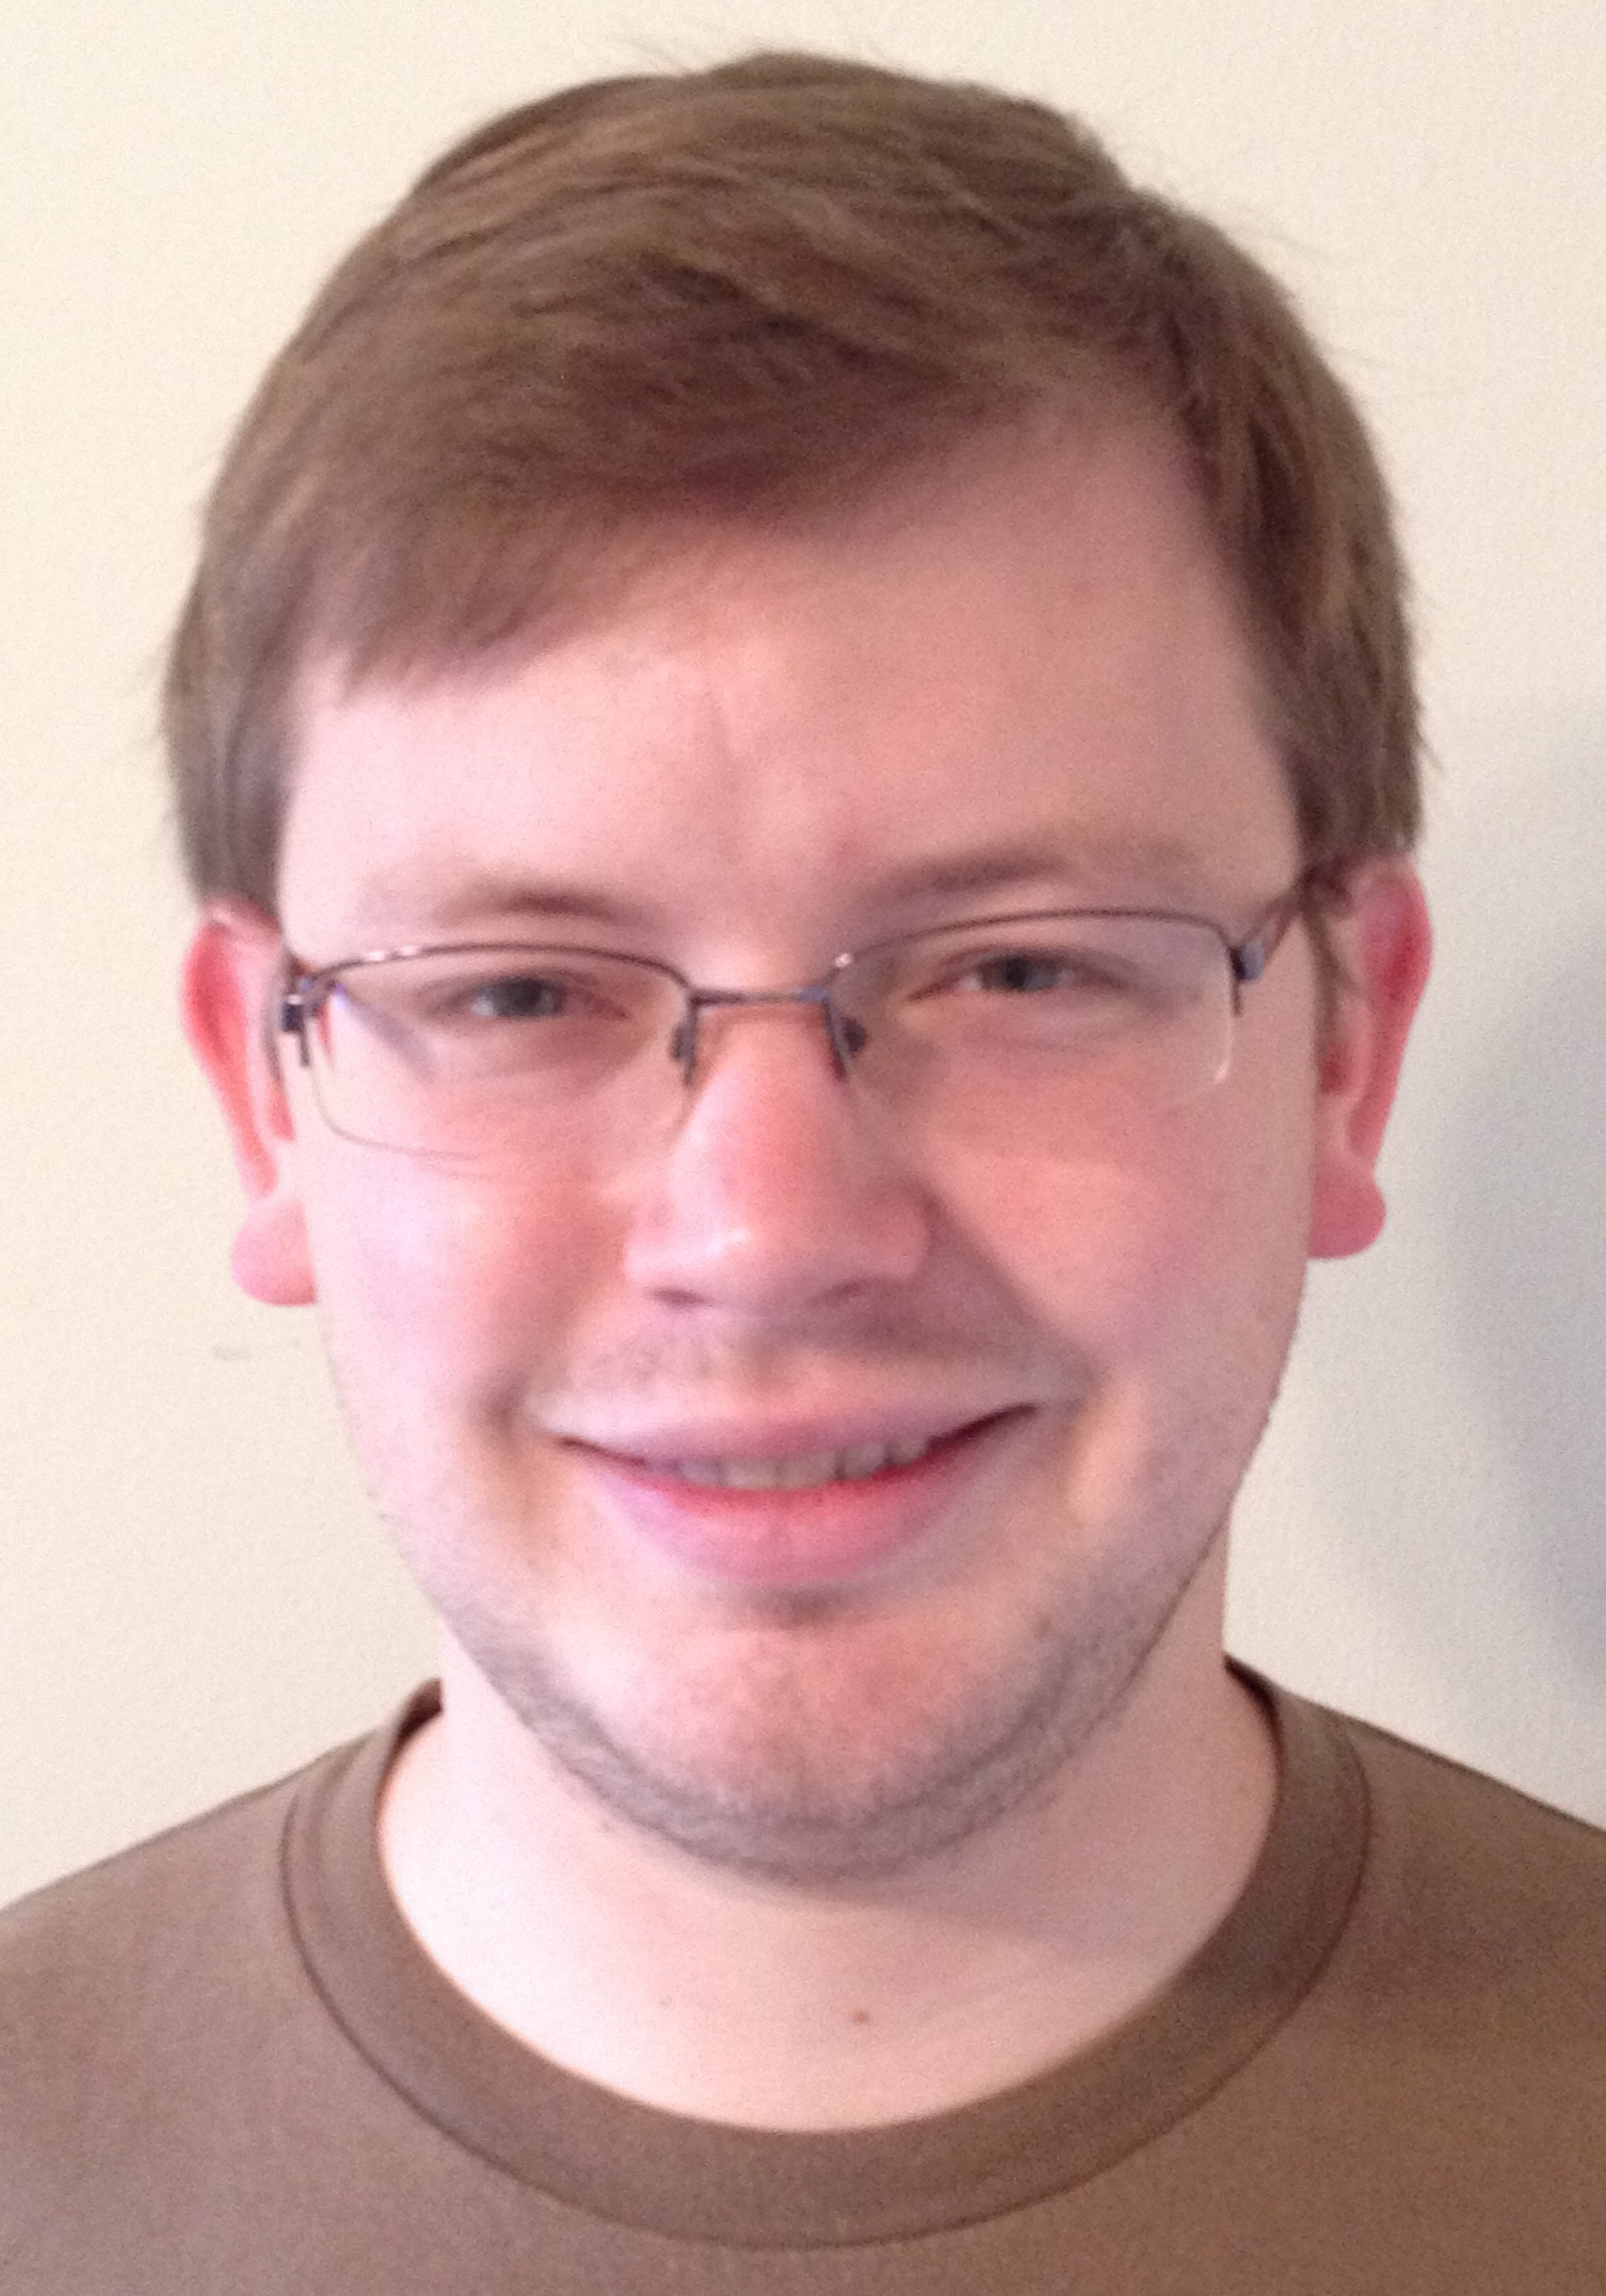
\includegraphics[width=1in,height=1.25in,clip,keepaspectratio]{john.jpg}}]{John Harrison}
  John Harrison is a graduate student researcher with Auburn University. He 
  works with Dr. Saad Biaz on a teaching tool for embedded operating systems. 
  John's research interests include embedded systems, robotics control systems 
  and compiler technologies.
  \end{IEEEbiography}
  
\end{document}
